\section{Modern Pseudorandom Number Generators}

While LFSRs and LFGs provide foundational algebraic methods for generating pseudorandom sequences, modern applications require generators that execute with minimal latency in software while exhibiting strong empirical statistical properties. This chapter explores two highly efficient families of generators: \textbf{Xorshift} (and its scrambled variants) and \textbf{PCG} (Permuted Congruential Generator).

\subsection{The Xorshift}

Introduced by George Marsaglia in 2003~\cite{marsaglia2003xorshift}, the Xorshift generator operates exclusively via hardware-efficient logical shift and bitwise XOR operations. Mathematically, it implements a linear transformation over the vector space $\mathbb{F}_2^w$, making it a software-efficient analogue of the LFSR.

\subsubsection{The Recurrence Relation}


Given a non-zero $w$-bit integer state $\mathbf{x}_n$, the subsequent state is generated by applying three successive shift-and-XOR operations using integer constants $a$, $b$, and $c$:
\begin{align*}
    \mathbf{y}_1 &= \mathbf{x}_0 \oplus (\mathbf{x}_0 \ll a) \\
    \mathbf{y}_2 &= \mathbf{y}_1 \oplus (\mathbf{y}_1 \gg b) \\
    \mathbf{x}_1 &= \mathbf{y}_2 \oplus (\mathbf{y}_2 \ll c)
\end{align*}


\subsubsection{Matrix Representation and Periodicity}
Rigorously, a $w$-bit word is a vector in $\mathbb{F}_2^w$. A left shift by $a$ positions equates to multiplying the state vector by a nilpotent $w \times w$ matrix $L^a$, where $L$ possesses ones on the first subdiagonal. Similarly, a right shift by $b$ is multiplication by $R^b = (L^T)^b$. Since XOR acts as standard vector addition over $\mathbb{F}_2$, the global state transition is governed by the linear map $\mathbf{x}_{n+1} = M\mathbf{x}_n$, where the transformation matrix $M$ is:
$$
M = (I + L^c)(I + R^b)(I + L^a)
$$

\begin{theorem}
An Xorshift generator defined by the state transition matrix $M$ over $\mathbb{F}_2^w$ has a maximal cycle length (period) of $2^w - 1$ if and only if $M$ has multiplicative order $2^w - 1$, equivalently if its minimal polynomial is primitive of degree $w$.
\end{theorem}
When the minimal polynomial is primitive, the state space partitions into exactly two cycles: a trivial fixed point at the zero vector (length 1), and a single maximum-length cycle containing all $2^w - 1$ non-zero states.

\subsubsection{Variants of the Xorshift}

Despite achieving maximum periodicity, pure linear Xorshift generators fail rigorous empirical statistical tests (e.g., \textit{MatrixRank} in TestU01). Because the transition function is linear over $\mathbb{F}_2$, consecutive outputs exhibit deterministically bounded matrix ranks and low-weight artifacts. To resolve this, "scrambled" variants append a non-linear output permutation to the linear state transition.


\begin{enumerate}
    \item \textbf{Xorshift*:} Appends a modular multiplication scrambler, $y_n \equiv (\mathbf{x}_{n+1} \cdot M_{\ast}) \pmod{2^w}$, to the linear state transition. This introduces non-linearity, significantly improving empirical statistical quality.

    \item \textbf{Xorshift+:} Expands the state space to multiple words and computes the output via modular addition: $y_n \equiv (\mathbf{s}_0 + \mathbf{s}_1) \pmod{2^w}$. However, because the initial carry-in is zero, the least significant bit remains strictly linear ($s_{0,0} \oplus s_{1,0}$), causing it to fail bit-reversed statistical tests.

    \item \textbf{Xoshiro (xor, shift, rotate) / Xoroshiro (xor, rotate, shift, rotate):} Integrates circular rotations into transition for faster bit diffusion across 128-bit or 256-bit states. It eliminates the lower-bit linearity flaw of Xorshift+ by utilizing dual-domain scramblers.
\end{enumerate}


\subsubsection{C++ Implementation of Xorshift}

The implementation of Xorshift follows the recurrence described above. The state is modified in-place by three shift-and-XOR operations. Each operation mixes bits from different positions, and the final state is returned as the output.

\cppfile[
    caption={Implementation of the Xorshift32 \texttt{next()} function},
    label={lst:xorshift32-next}
]{codes/xorshift/xorshift32_next.cpp}

A scrambled variant, Xorshift*, uses the same type of linear state transition but multiplies the final state by a fixed odd constant. This multiplication is not linear over $\mathbb{F}_2$ and therefore improves the visible output quality.

\cppfile[
    caption={Implementation of the Xorshift* \texttt{next()} function},
    label={lst:xorshiftstar-next}
]{codes/xorshift/xorshift_star64_next.cpp}

\subsubsection{Experimental Comparison of Xorshift}

Three variants were tested. The first one uses the classical shift parameters $(13,17,5)$. The second one uses a non-standard set of shifts, still over a large 32-bit range, but with weaker mixing. The third one changes only one shift parameter: the last shift is changed from $5$ to $1$. This keeps the generator non-trivial and still operating over the full 32-bit range, but it weakens the bit mixing.

\begin{table}[htbp]
\centering
\small
\resizebox{\textwidth}{!}{%
\begin{tabular}{|l|r|r|r|r|}
\hline
Variant & Seed & Shift $a$ & Shift $b$ & Shift $c$ \\
\hline
Good Xorshift32 & $2463534242$ & $13$ & $17$ & $5$ \\
Bad large-range Xorshift32 & $2463534242$ & $31$ & $1$ & $31$ \\
One weak-shift Xorshift32 & $2463534242$ & $13$ & $17$ & $1$ \\
\hline
\end{tabular}%
}
\caption{Xorshift parameter sets used in the experiment}
\label{tab:xorshift-parameters}
\end{table}

\begin{table}[htbp]
\centering
\small
\resizebox{\textwidth}{!}{%
\begin{tabular}{|l|r|r|r|r|r|r|}
\hline
Variant & Min & Max & Mean & Std. dev. & One-bit ratio & $\chi^2$ \\
\hline
Good Xorshift32 & $95953$ & $4294949870$ & $2149746614.22$ & $1242030056.19$ & $0.500326$ & $21.6532$ \\
Bad large-range Xorshift32 & $469467027$ & $3988719432$ & $2426824957.03$ & $1045875667.31$ & $0.519531$ & $130468.7500$ \\
One weak-shift Xorshift32 & $89687$ & $4294910162$ & $2144856443.53$ & $1238218476.87$ & $0.499973$ & $19.0068$ \\
\hline
\end{tabular}%
}
\caption{Basic Xorshift statistics computed from $100000$ outputs}
\label{tab:xorshift-statistics}
\end{table}

The good Xorshift32 variant has a mean close to the middle of the 32-bit output range and a one-bit ratio close to $0.5$. The histogram chi-square value is also moderate, which suggests that the one-dimensional distribution is reasonably balanced in this simple test.

The bad large-range variant is not a toy constant example: it still operates on 32-bit values. However, the shift parameters $(31,1,31)$ mix bits poorly. This is visible in the histogram and in the bit ratio, which is noticeably shifted away from the ideal value $0.5$.

The one weak-shift variant changes only the last shift from $5$ to $1$. The basic statistics remain close to the good generator, which shows that a single simple experiment may fail to expose a weaker parameter choice. This case is useful as a warning: not every bad parameter choice produces an immediately absurd plot.

\begin{figure}[htbp]
\centering
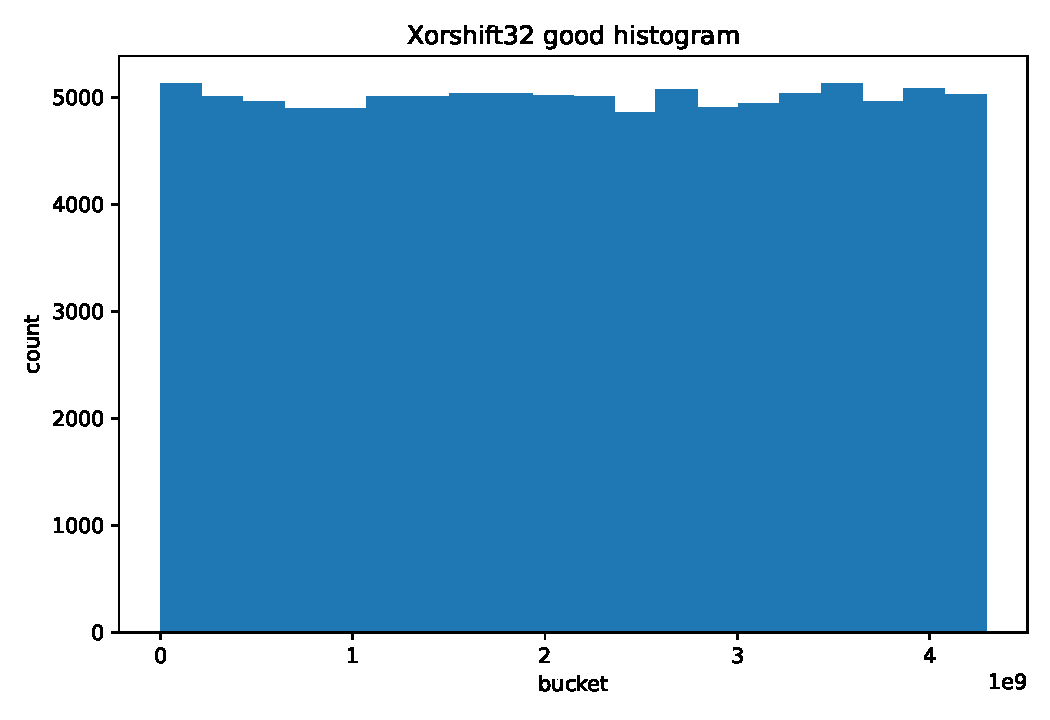
\includegraphics[width=0.48\textwidth]{figures/xorshift/good/xorshift_good_histogram.pdf}
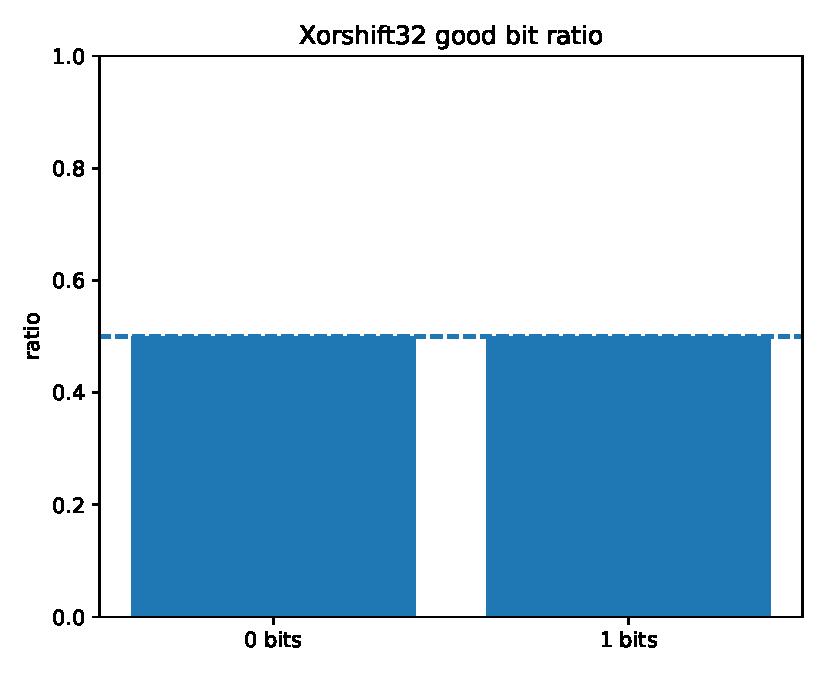
\includegraphics[width=0.48\textwidth]{figures/xorshift/good/xorshift_good_bit_ratio.pdf}
\caption{Histogram and bit ratio for the good Xorshift32 generator}
\label{fig:xorshift-good-hist-bits}
\end{figure}

Figure \ref{fig:xorshift-good-hist-bits} shows that the good variant distributes values relatively evenly across buckets and keeps the bit ratio close to the ideal value $0.5$.

\begin{figure}[htbp]
\centering
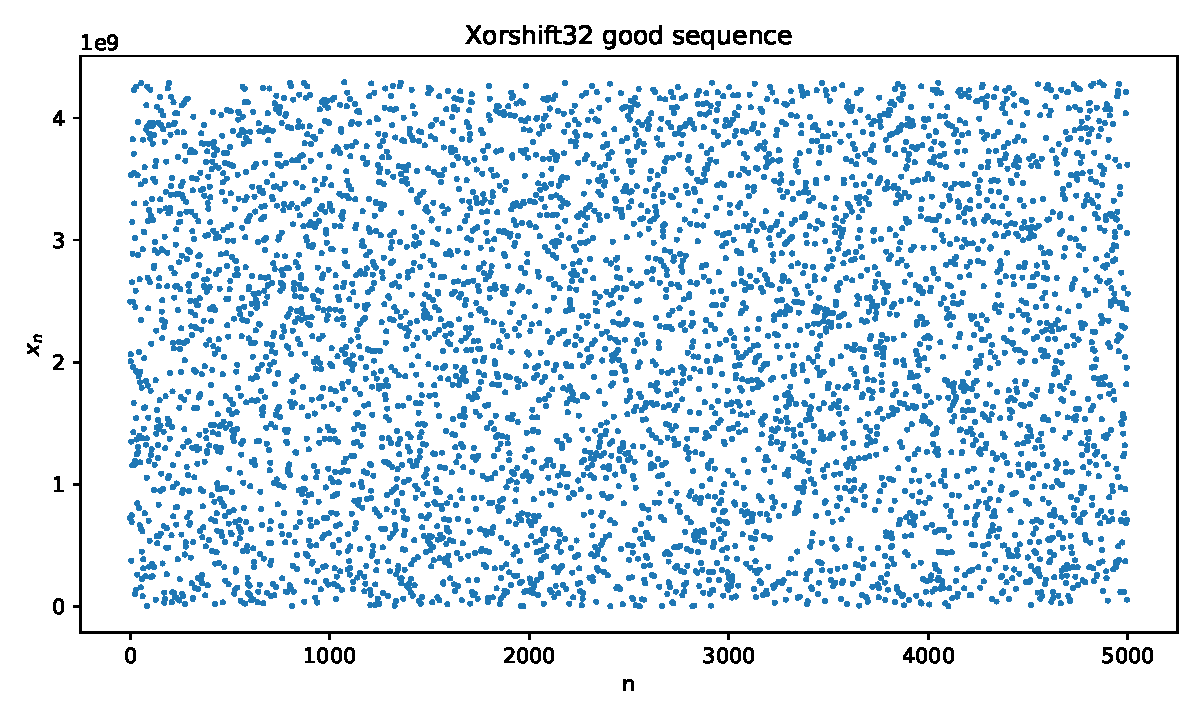
\includegraphics[width=0.48\textwidth]{figures/xorshift/good/xorshift_good_sequence.pdf}
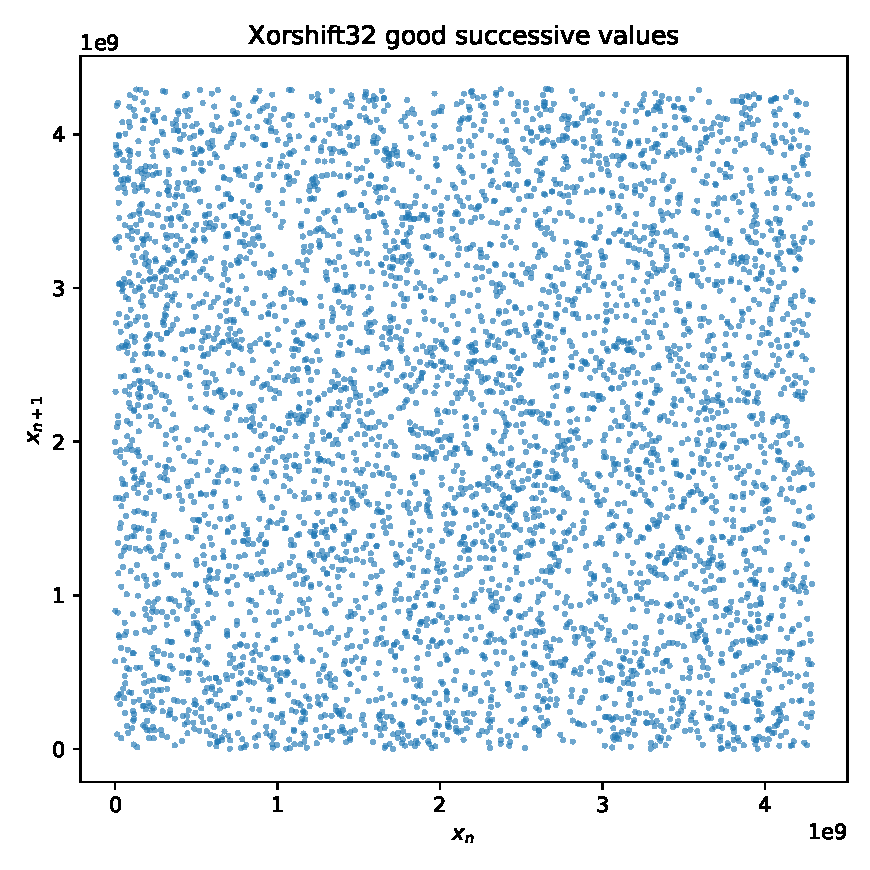
\includegraphics[width=0.48\textwidth]{figures/xorshift/good/xorshift_good_successive_values.pdf}
\caption{Sequence plot and successive-value plot for the good Xorshift32 generator}
\label{fig:xorshift-good-seq}
\end{figure}

Figure \ref{fig:xorshift-good-seq} shows that the generated values cover the output range. However, this does not prove full statistical quality, because pure Xorshift remains linear over $\mathbb{F}_2$.

\begin{figure}[htbp]
\centering
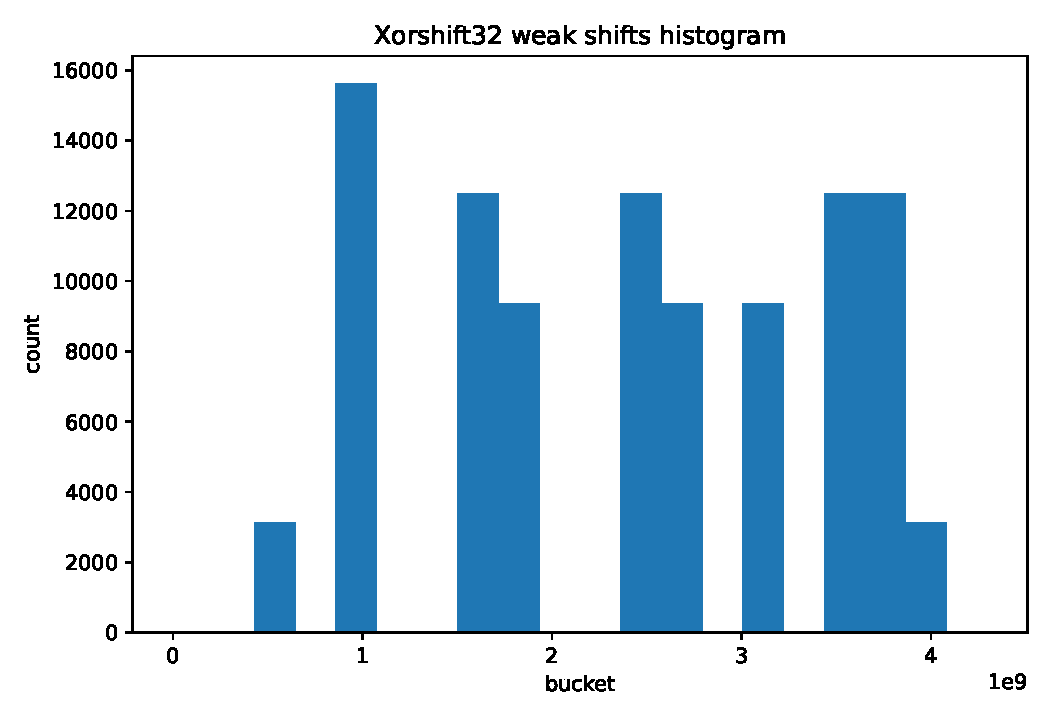
\includegraphics[width=0.48\textwidth]{figures/xorshift/bad_large_range/xorshift_bad_large_range_histogram.pdf}
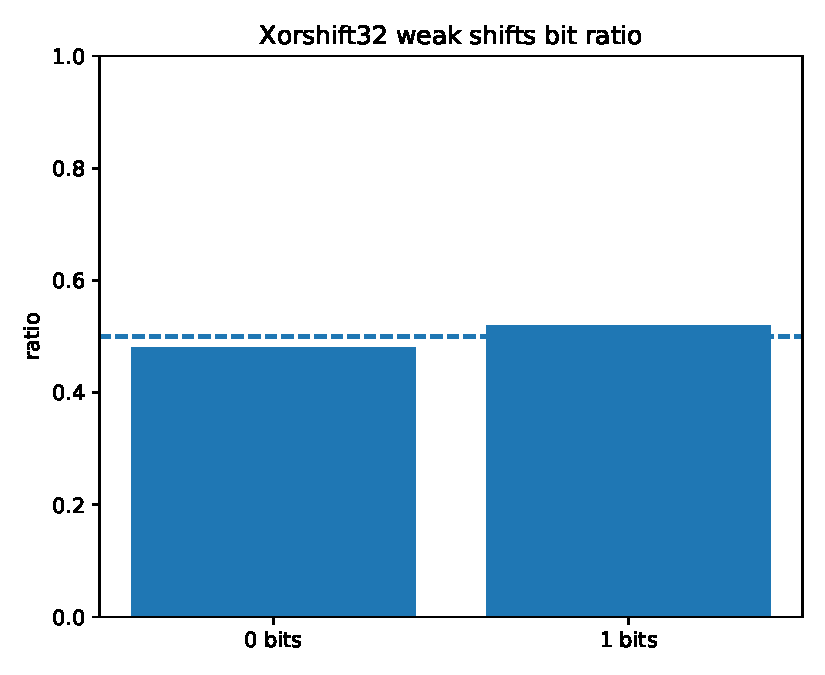
\includegraphics[width=0.48\textwidth]{figures/xorshift/bad_large_range/xorshift_bad_large_range_bit_ratio.pdf}
\caption{Histogram and bit ratio for the bad large-range Xorshift32 generator}
\label{fig:xorshift-bad-hist-bits}
\end{figure}

Figure \ref{fig:xorshift-bad-hist-bits} shows the weaker $(31,1,31)$ shift choice. Unlike the zero-state example, this generator still produces values over a large range, but the bucket distribution and bit ratio are visibly worse than for the standard parameters.

\begin{figure}[htbp]
\centering
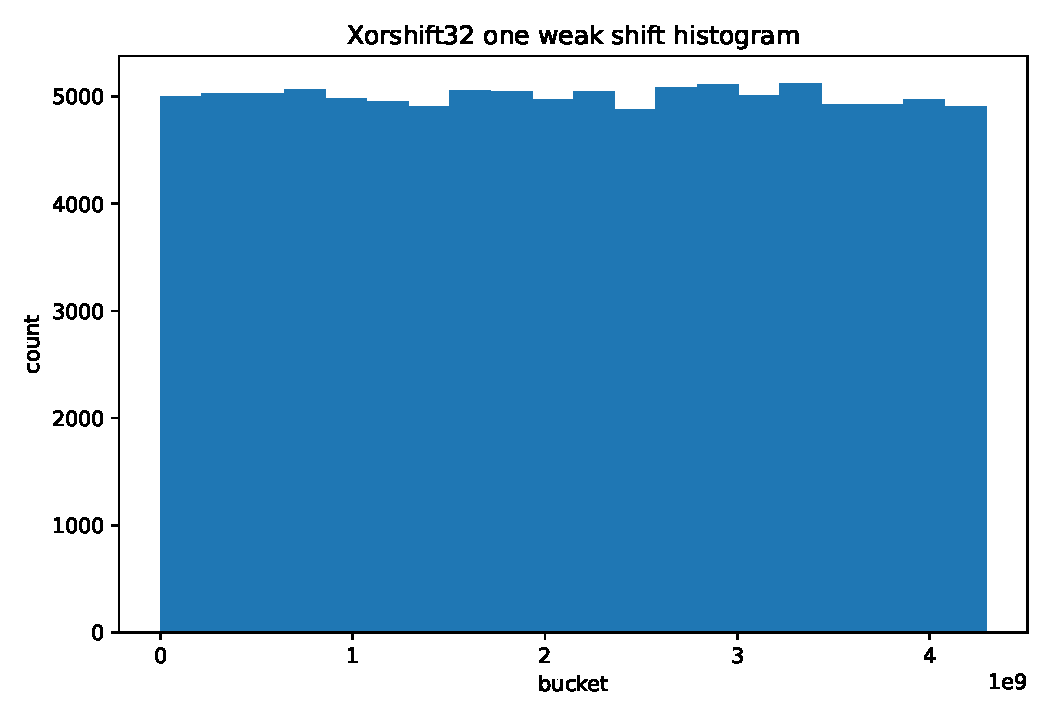
\includegraphics[width=0.48\textwidth]{figures/xorshift/single_bad_parameter/xorshift_single_bad_parameter_histogram.pdf}
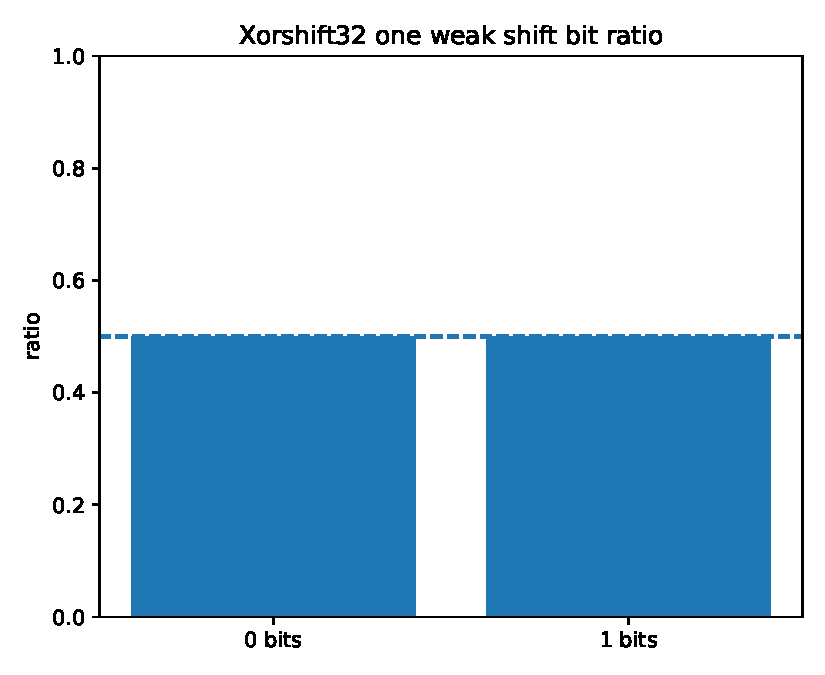
\includegraphics[width=0.48\textwidth]{figures/xorshift/single_bad_parameter/xorshift_single_bad_parameter_bit_ratio.pdf}
\caption{Histogram and bit ratio for the one weak-shift Xorshift32 generator}
\label{fig:xorshift-zero-hist-bits}
\end{figure}

Figure \ref{fig:xorshift-zero-hist-bits} shows the case where only one shift parameter was changed. The plot does not collapse, but this is precisely the point: a visually acceptable short run is not enough to prove that the selected transition matrix has maximal period or good empirical behavior.



\subsection{The PCG}

Introduced by Melissa E. O'Neill in 2014~\cite{oneill2014pcg}, the PCG framework operates exclusively via hardware-efficient modular arithmetic and bitwise permutation operations. Mathematically, it implements a non-linear transformation over the ring $\mathbb{Z}/2^k\mathbb{Z}$, making it an empirically stronger alternative to classical LCG.


\subsubsection{Representation and Periodicity}

The core engine of PCG is an affine recurrence relation operating over the integer ring $\mathbb{Z}/2^k\mathbb{Z}$:
$$
S_{n+1} \equiv (a S_n + c) \pmod{2^k}
$$
By choosing a multiplier $a \equiv 1 \pmod 4$ and an odd increment $c$, the generator guarantees an unbroken maximal cycle of length $2^k$.

Crucially, the increment $c$ uniquely defines the \textit{stream} of the generator. Because any odd $c$ yields a full period, a $k$-bit state space allows for exactly $2^{k-1}$ distinct streams. This cycle topology permits developers to assign distinct streams (via different constants $c$) to parallel threads, mathematically guaranteeing distinct state trajectories for different streams.


\subsubsection{Popular variants of the PCG Framework}

Despite achieving maximum periodicity, pure linear congruential generators fail rigorous empirical statistical tests (e.g., \textit{Spectral Test} in TestU01). To resolve this issue, "permuted" variants append a non-linear output permutation to the affine state transition.

\begin{enumerate}
    \item \textbf{PCG-XSH-RR:} Uses a random rotation scrambler, $u_n = \text{ROTR}(X, r)$. This introduces non-linear bit diffusion, significantly improving empirical statistical quality.

    \item \textbf{PCG-XSH-RS:} Reduces the permutation operations to a simple random shift and computes the output via logical right shifts: $u_n = X \gg r$. However, because it avoids circular rotation, the lowest bits remain partially correlated to the state, causing it to fail some bit-reversed statistical tests.

    \item \textbf{PCG-RXS-M-XS ("random xorshift, multiply, xorshift"):} Integrates an internal 64-bit multiplication into the permutation for faster bit diffusion across 32-bit or 64-bit states. 
\end{enumerate}


\subsubsection{C++ Implementation of PCG}

The PCG generator combines an LCG-style internal state transition with an output permutation. First, the internal 64-bit state is advanced using an affine recurrence. Then the old state is transformed using xorshift and rotation operations to produce a 32-bit output.

\cppfile[
    caption={Implementation of the PCG32 \texttt{next()} function},
    label={lst:pcg32-next}
]{codes/pcg/pcg32_next.cpp}

This separation between the state transition and the output function is the main idea of PCG. The internal transition gives a long period when the multiplier and increment satisfy the required conditions, while the permutation hides the linear structure of the underlying congruential sequence.

\subsubsection{Experimental Comparison of PCG}

Three PCG variants were tested. The first one uses the standard multiplier and an odd increment, so it satisfies the full-period condition for the affine recurrence modulo $2^{64}$. The second one uses an even increment. The third one uses zero increment, turning the transition into a purely multiplicative recurrence.

\begin{table}[htbp]
\centering
\small
\resizebox{\textwidth}{!}{%
\begin{tabular}{|l|r|r|r|}
\hline
Variant & Seed & Multiplier & Increment \\
\hline
Good PCG32 & $42$ & $6364136223846793005$ & $109$ \\
Bad large-range PCG32 & $42$ & $6364136223846793005$ & $54$ \\
Zero-increment PCG32 & $42$ & $6364136223846793005$ & $0$ \\
\hline
\end{tabular}%
}
\caption{PCG parameter sets used in the experiment}
\label{tab:pcg-parameters}
\end{table}

\begin{table}[htbp]
\centering
\small
\resizebox{\textwidth}{!}{%
\begin{tabular}{|l|r|r|r|r|r|r|}
\hline
Variant & Min & Max & Mean & Std. dev. & One-bit ratio & $\chi^2$ \\
\hline
Good PCG32 & $0$ & $4294958997$ & $2144931975.79$ & $1239128951.68$ & $0.499635$ & $16.2216$ \\
Bad large-range PCG32 & $0$ & $4294960179$ & $2146754647.86$ & $1238184206.83$ & $0.500030$ & $26.4868$ \\
Zero-increment PCG32 & $0$ & $4294954284$ & $2147657129.78$ & $1239210617.46$ & $0.499794$ & $12.4160$ \\
\hline
\end{tabular}%
}
\caption{Basic PCG statistics computed from $100000$ outputs}
\label{tab:pcg-statistics}
\end{table}

The good PCG32 variant has a balanced bit ratio and a histogram close to uniform in this experiment. The output permutation makes the generator look much less directly tied to the linear congruential state transition.

The even-increment and zero-increment variants still produce values over a large range in a short test, so their histograms may look deceptively acceptable. However, they violate the usual full-period requirement that the increment should be odd. Therefore, their problem is not necessarily visible in every short plot, but it is structural.

\begin{figure}[htbp]
\centering
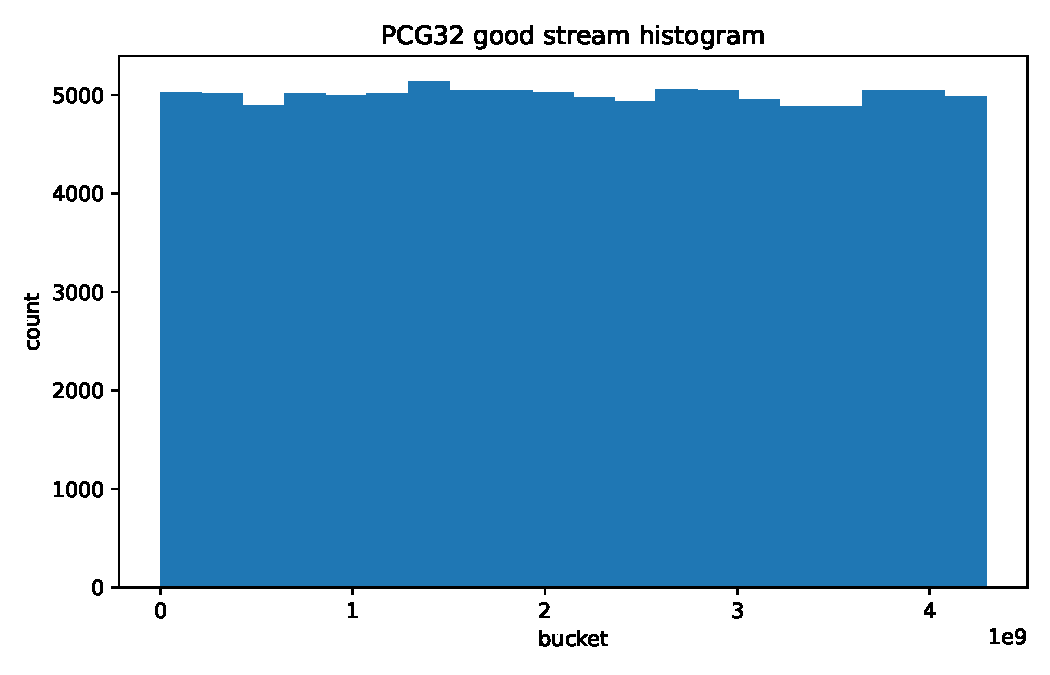
\includegraphics[width=0.48\textwidth]{figures/pcg/good/pcg_good_histogram.pdf}
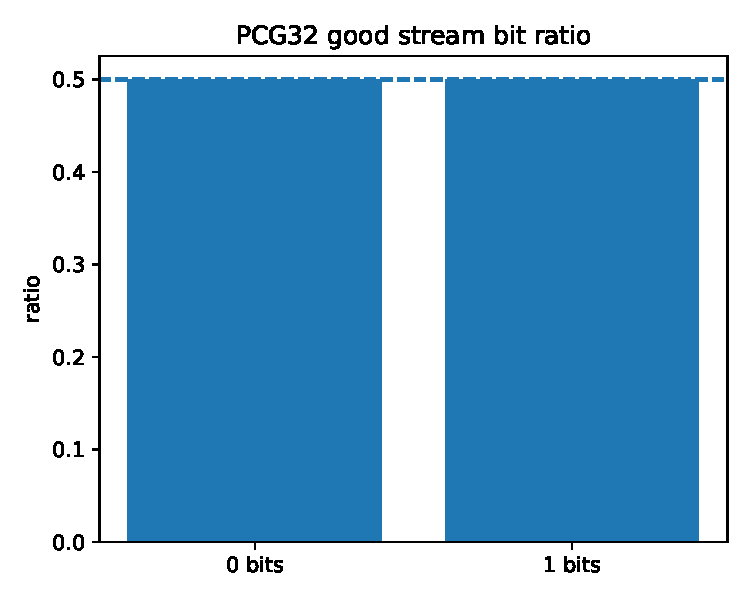
\includegraphics[width=0.48\textwidth]{figures/pcg/good/pcg_good_bit_ratio.pdf}
\caption{Histogram and bit ratio for the good PCG32 generator}
\label{fig:pcg-good-hist-bits}
\end{figure}

Figure \ref{fig:pcg-good-hist-bits} shows a balanced one-dimensional distribution and a bit ratio close to $0.5$.

\begin{figure}[htbp]
\centering
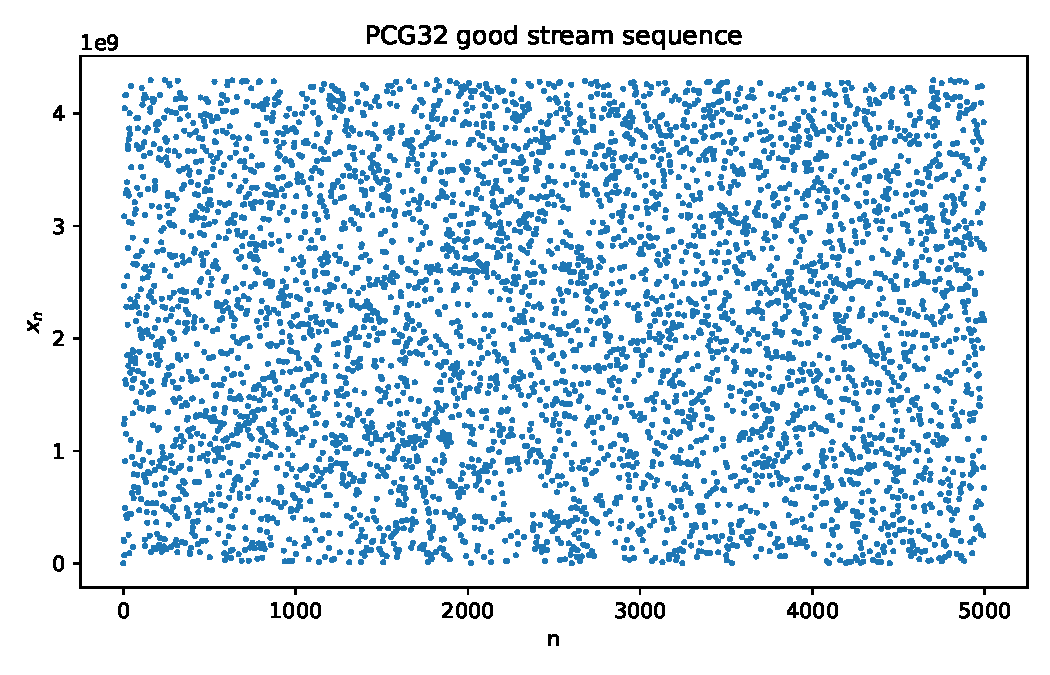
\includegraphics[width=0.48\textwidth]{figures/pcg/good/pcg_good_sequence.pdf}
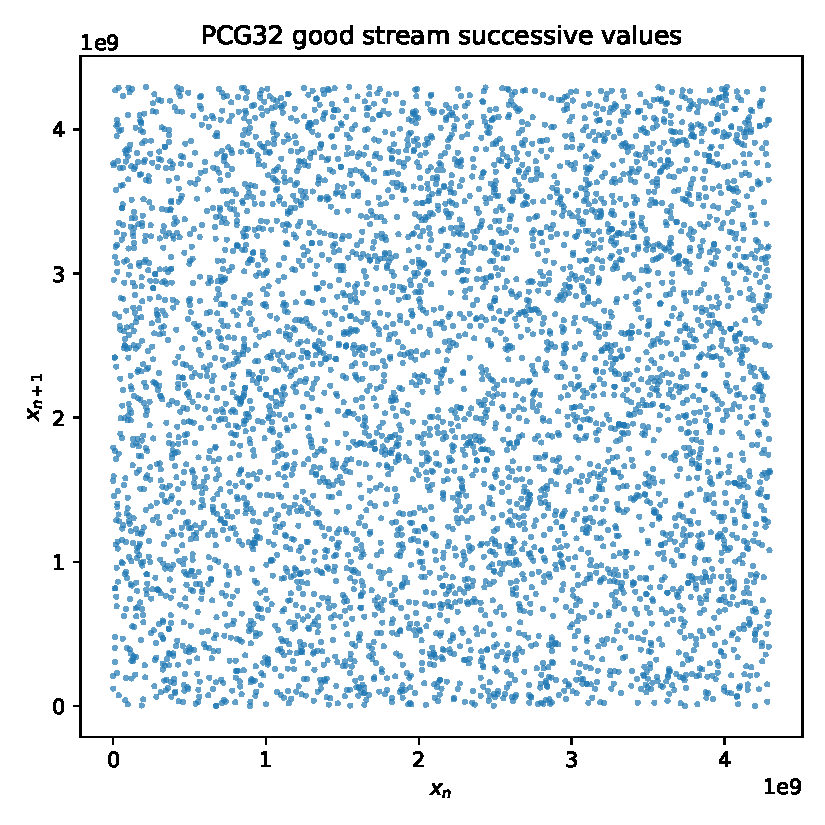
\includegraphics[width=0.48\textwidth]{figures/pcg/good/pcg_good_successive_values.pdf}
\caption{Sequence plot and successive-value plot for the good PCG32 generator}
\label{fig:pcg-good-seq}
\end{figure}

Figure \ref{fig:pcg-good-seq} shows that consecutive outputs cover the square of possible values without collapsing into a trivial pattern.

\begin{figure}[htbp]
\centering
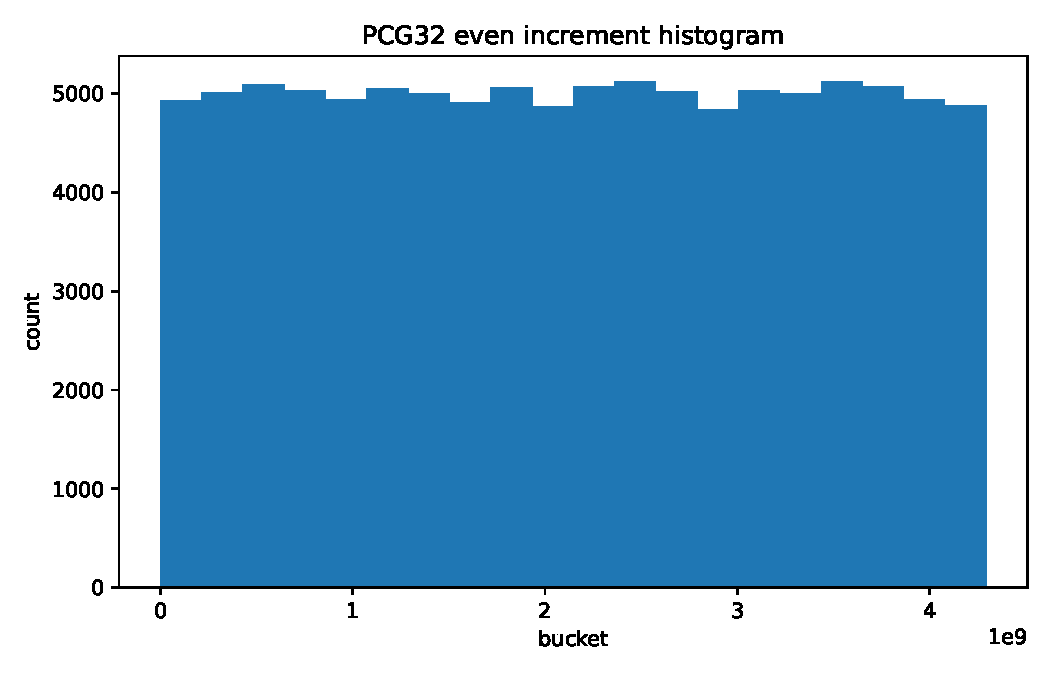
\includegraphics[width=0.48\textwidth]{figures/pcg/bad_large_range/pcg_bad_large_range_histogram.pdf}
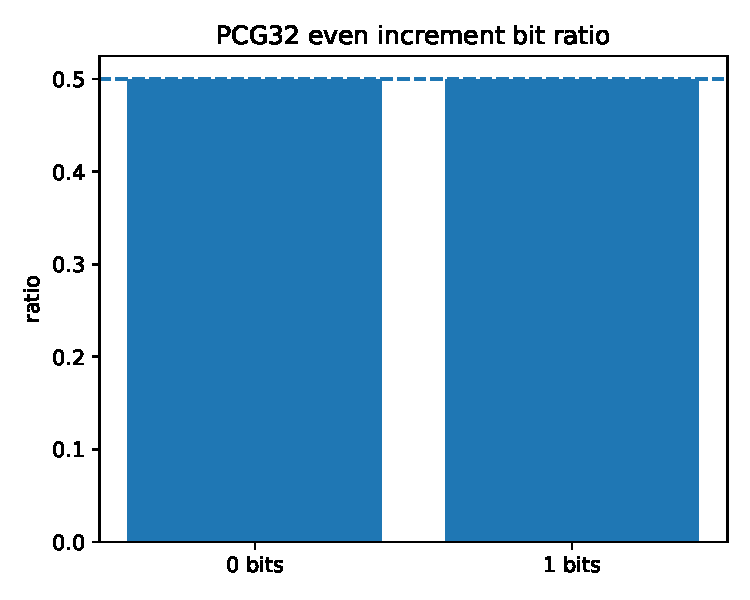
\includegraphics[width=0.48\textwidth]{figures/pcg/bad_large_range/pcg_bad_large_range_bit_ratio.pdf}
\caption{Histogram and bit ratio for the even-increment PCG32 generator}
\label{fig:pcg-bad-hist-bits}
\end{figure}

Figure \ref{fig:pcg-bad-hist-bits} demonstrates that a generator with a broken period condition may still look acceptable in simple empirical tests. This is why theoretical conditions are necessary in addition to plots.

\begin{figure}[htbp]
\centering
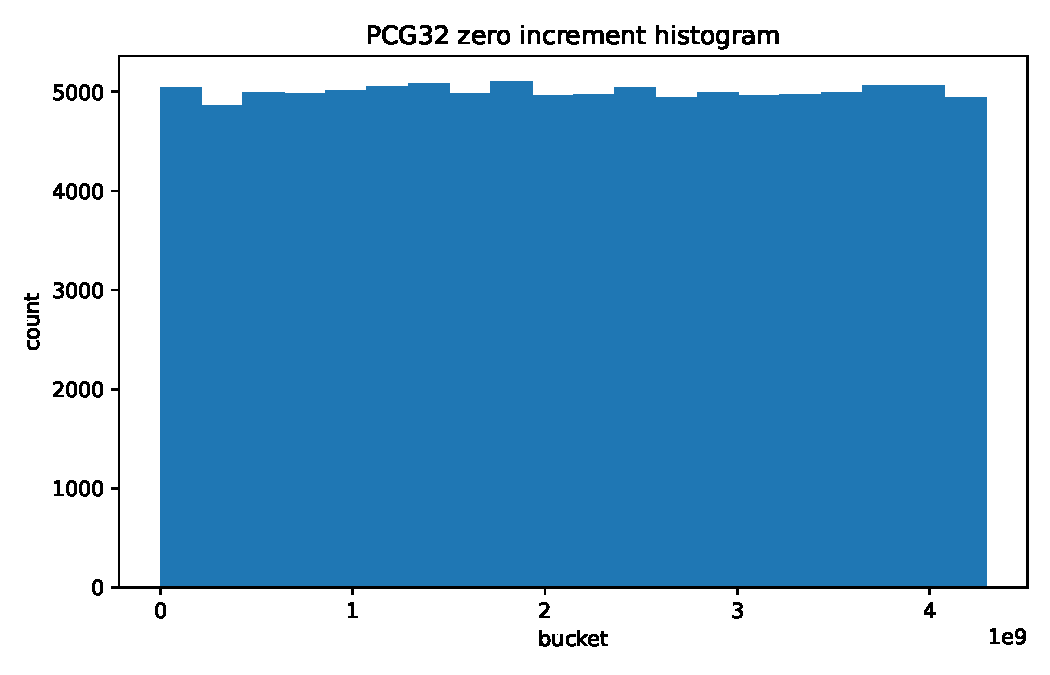
\includegraphics[width=0.48\textwidth]{figures/pcg/single_bad_parameter/pcg_single_bad_parameter_histogram.pdf}
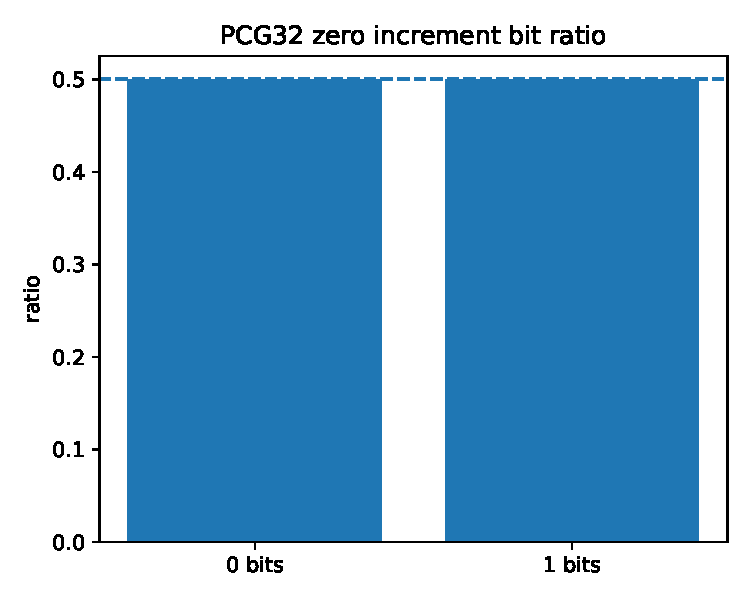
\includegraphics[width=0.48\textwidth]{figures/pcg/single_bad_parameter/pcg_single_bad_parameter_bit_ratio.pdf}
\caption{Histogram and bit ratio for the zero-increment PCG32 generator}
\label{fig:pcg-zero-hist-bits}
\end{figure}

Figure \ref{fig:pcg-zero-hist-bits} shows the variant with zero increment. The short-range statistics may still look surprisingly normal, but the recurrence no longer has the full PCG cycle structure. This is another example where empirical plots alone can be too weak as a correctness criterion.

Overall, the experiments show that modern generators can hide many defects in short one-dimensional tests. Xorshift exposes the zero-state problem immediately, while PCG can appear visually reasonable even with broken period conditions. Therefore, both implementation details and theoretical parameter constraints remain essential.
